\documentclass[french, a4paper, 12pt, titlepage]{article}
%% Peut remplacer "article" par "scrartcl" %%

\usepackage{a4wide}
%\usepackage[top=2cm, bottom=2cm, left=2cm, right=2cm]{geometry}
\raggedbottom % prevents vertical white space on pages that cannot be filled properly

\usepackage{hyperref}
\hypersetup{
	colorlinks=true,       	% false: boxed links; true: colored links
	linkcolor=black,          	% color of internal links
	urlcolor=blue,           	% color of external links
	citecolor=grey
}

\usepackage[T1]{fontenc}
%\usepackage{fourier}
%\usepackage{utopia}
%\usepackage{palatino}

\usepackage{lmodern}
%% ajouter fonte petite capitale grasse à lmodern avec celle de computer modern %%
\rmfamily
\DeclareFontShape{T1}{lmr}{b}{sc}{<->ssub*cmr/bx/sc}{}
\DeclareFontShape{T1}{lmr}{bx}{sc}{<->ssub*cmr/bx/sc}{}
%% /ajout %%
\usepackage{wrapfig}

%\usepackage[a4paper]{geometry} % marges plus petites que a4paper standard
\usepackage{listings} % insérer code source
%\usepackage{algorithm} % algorithmique
%\usepackage{algorithmic}
\usepackage{url}
\usepackage[usenames, dvipsnames]{color} % couleurs (nombre de base étendu)
\usepackage{graphicx} % insérer images
\usepackage[utf8]{inputenc}
\usepackage[french]{babel}
\usepackage{amsmath}
\usepackage{amsfonts}
\usepackage{amssymb}
\usepackage{amsthm}
\usepackage{multicol}
\definecolor{grey}{rgb}{0.96,0.96,0.96}
\definecolor{grey2}{rgb}{0.3,0.3,0.3}

%% Define listings params %%
\lstset{
	numbers=left,
	language=Java,
	tabsize=4,
	frame=single, % cadre autour du code
	breaklines=true, % autorise couper ligne trop longue
	basicstyle=\small\ttfamily,
	numberstyle=\scriptsize\ttfamily,
	backgroundcolor=\color{grey},
	showstringspaces=false,
	keywordstyle=\color{OliveGreen},
	stringstyle=\color{BrickRed},
	commentstyle=\color{grey2}\it,
	stepnumber=1
} % numérote toute les x lignes
% listing utf8 fr %
\lstset{%
	inputencoding=utf8,
	extendedchars=true,
	literate=
		{é}{{\'{e}}}1
		{è}{{\`{e}}}1
		{ê}{{\^{e}}}1
		{ë}{{\¨{e}}}1
		{û}{{\^{u}}}1
		{ù}{{\`{u}}}1
		{â}{{\^{a}}}1
		{à}{{\`{a}}}1
		{î}{{\^{i}}}1
		{ç}{{\c{c}}}1
		{Ç}{{\c{C}}}1
		{É}{{\'{E}}}1
		{Ê}{{\^{E}}}1
		{À}{{\`{A}}}1
		{Â}{{\^{A}}}1
		{Î}{{\^{I}}}1
}
%% /Define listings params %%

%% Francisation des algorithmes
%\renewcommand{\algorithmicrequire} {\textbf{\textsc{Entrées:}}}
%\renewcommand{\algorithmicensure}  {\textbf{\textsc{Sorties:}}}
%\renewcommand{\algorithmicwhile}   {\textbf{tant que}}
%\renewcommand{\algorithmicdo}      {\textbf{faire}}
%\renewcommand{\algorithmicendwhile}{\textbf{fin tant que}}
%\renewcommand{\algorithmicend}     {\textbf{fin}}
%\renewcommand{\algorithmicif}      {\textbf{si}}
%\renewcommand{\algorithmicendif}   {\textbf{fin si}}
%\renewcommand{\algorithmicelse}    {\textbf{sinon}}
%\renewcommand{\algorithmicthen}    {\textbf{alors}}
%\renewcommand{\algorithmicfor}     {\textbf{pour}}
%\renewcommand{\algorithmicforall}  {\textbf{pour tout}}
%\renewcommand{\algorithmicdo}      {\textbf{faire}}
%\renewcommand{\algorithmicendfor}  {\textbf{fin pour}}
%\renewcommand{\algorithmicloop}    {\textbf{boucler}}
%\renewcommand{\algorithmicendloop} {\textbf{fin boucle}}
%\renewcommand{\algorithmicrepeat}  {\textbf{répéter}}
%\renewcommand{\algorithmicuntil}   {\textbf{jusqu'à}}
%\renewcommand{\algorithmiccomment} {\STATE //}
%\newcommand{\BEGIN}{\STATE \fbox{Début}}
%\newcommand{\END}{\STATE \fbox{Fin}}
%\floatname{algorithm}{Algorithme}
%% /francisation des algorithmes

\renewcommand{\qedsymbol}{}

\newcommand{\petit}[1]{
	\medskip \noindent
	\begin{small}
	#1)
	\end{small}
}

\newcommand{\graph}[2]{
\medskip
	\begin{center}
		\includegraphics[scale=#1]{#2}
	\end{center}
\medskip
}

\begin{document}

\title{Atelier Systèmes d'Exploitation\\Simulation Interbancaire}
\author{\textsc{Martel} Damien}
\date{Compilé le \today}

\maketitle
%% Laisse page blanche pour verso page de garde %%

\vfill
\pagebreak

%\tableofcontents
\newpage
\strut\thispagestyle{empty}
\vfill
\pagebreak
\tableofcontents
\strut\thispagestyle{empty}
%\setcounter{page}{0}
\newpage
\setcounter{page}{1}

\section{Schéma général de la simulation}
\medskip
\begin{center}
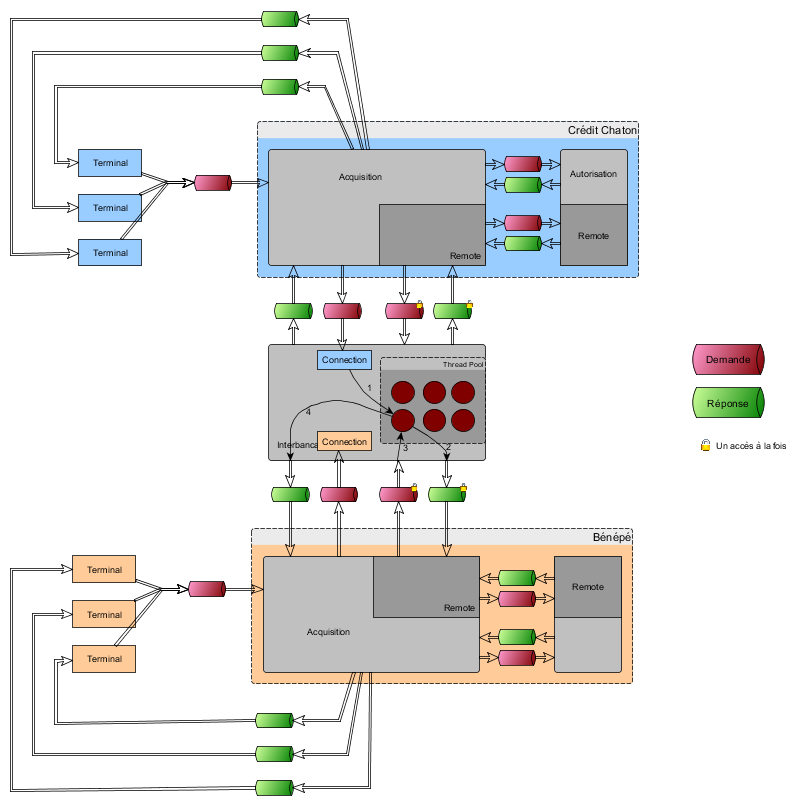
\includegraphics[scale=0.5]{global}
\end{center}
\medskip

Tout au long de ce manuel, nous utiliserons la notion de connexion local et distante.
Une connexion local signifie qu'un terminal associé à une banque émet une demande pour un débit sur un compte de cette même banque (terminal crédit chaton utilisé par un client de crédit chaton), alors qu'une connexion distante ce réfère à un client utilisant un terminal associé à une autre banque (client de la bénépé utilisant un terminal de crédit chaton).
Ces deux cas traiter par le même serveur d'acquisition sont router différemment et passe par deux partie différente de l'application.

\section{Serveurs mis en place}
Pour cette simulation, un minimum de 3 serveurs sont nécessaire afin d'effectuer des transaction local
(un client utilisant un terminal de sa banque),
2 serveurs supplémentaire par client de banque différent pour les transaction à distance (un client utilisant le terminal d'une autre banque que la sienne).

Les 3 serveurs permettant les connexions locales sont les suivant:

\begin{itemize}
	\item Terminal
	\item Acquisition
	\item Autorisation
\end{itemize}

Afin de permettre un connexion distante, il faut rajouter pour cela le serveur Interbancaire, connecté a un autre couple de serveur Acquisition/Autorisation associé à une banque.

\section{Déroulement d'une transaction}
\subsection{Local}
En utilisant un terminal de sa propre banque, une demande et effectué au serveur d'acquisition qui retransmettra l'information au serveur d'autorisation.
Une fois cette demande traité, le serveur d'autorisation renverra au serveur d'acquisition la réponse qui pourra signaler au terminal, à l'aide d'un tube dédié.
\medskip
\begin{center}
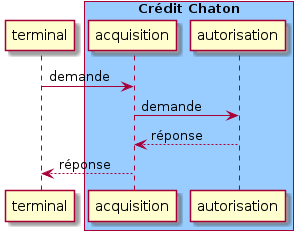
\includegraphics[scale=0.7]{transactionLocal}
\end{center}
\medskip

\subsection{Distante}
Pour l'utilisation d'un terminal d'une autre banque, le chemin est légèrement plus long.
Le serveur d'acquisition, qui récupère une demande avec un identifiant de banque différent du sien, enverra la demande au serveur interbancaire à travers un tube qui lui est propre.\\
\noindent
Le serveur interbancaire possède pour chaque tube relié à une banque, un thread s'occupant d'encapsuler la demande en y rajoutant, la banque émettant la demande, la banque à laquelle est destiné cette demande ainsi que la demande en elle même avant de l'envoyer a travers un tube relié à la partie centrale du serveur s'occupant de router ces demande, d'en attendre la réponse et la renvoyer à la bonne banque.
Cette partie est implementé sous la forme d'une piscine de processus léger (thread pool) dont le nombre limite la quantité de demande simultané qu'elle peut traiter.\\
\noindent
Les serveur d'acquisition disposent ainsi d'un deuxième chemin d'accès a leurs serveur d'autorisation différenciant les demande émise par un terminal associé à leurs banque ou provenant du serveur interbancaire, leurs permettant de renvoyer des réponses distante au serveur interbancaire.
\medskip
\begin{center}
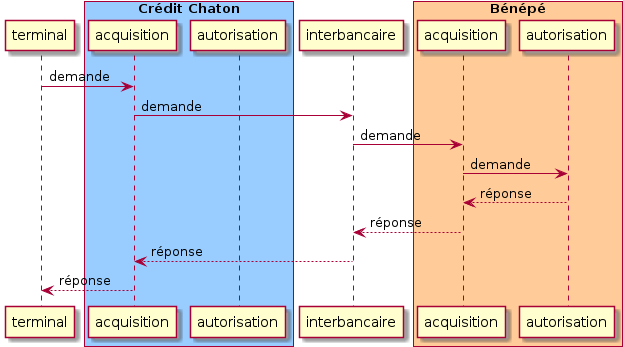
\includegraphics[scale=0.6]{transactionDistante}
\end{center}
\medskip

\section{Arbre des processus}
\graph{0.6}{arbre}
Chaque serveur se lancent de manière indépendante, et n'ont pas de lien de parenté direct, ils utilisent donc pour communiquer des tubes nommé en respectant une certaine convention de nommage.\\
\noindent
Afin de pouvoir lancer chaque processus dans l'ordre que l'on veut, ils essayerons tous de créer le tube afin d'éviter des erreur de l'ordre de \og No such file or directory \fg\\
\noindent
Enfin, si les processus doivent effectuer plusieurs actions de manière asynchrone, ils créerons des threads dont le nombre ne sera limité que si nécessaire,
c'est à dire que dans une logique de parallélisation, la création de plus de threads sert a exécuter la même action (comme dans le serveur interbancaire) au lieu d'effectuer une autre action légèrement différente (comme dans le serveur d'acquisition).\\
\noindent
Ainsi le parallélisme n'est pas obtenu en augmentant un paramètre déterminant la quantité de ressource alloué au processus (nombre de thread) mais l'exécution d'un nouveau serveur.\\
\noindent
Sauf pour le serveur Interbancaire, goulot d'étranglement des messages qui ne dispose pas à ce jour de design lui permettant cela.


\section{Communication}
Afin de pouvoir communiquer ensemble, et ne possédant pas de lien filiale, les différent serveur communique a l'aide de tube nommée, et pour garantir leurs communication, une certaine convention à été utilisé.\\
\noindent
Nous présenterons ici les chemins utilisé pour les différent tubes, afin de pouvoir différentier les différent serveurs associé aux banques, on peut parfois retrouver dans le nom un mot entre chevrons (\og <id> \fg) ceci signifie que le serveur doit le remplacer par la donnée correspondante (par exemple: <bankId> signifie que le serveur doit remplacer dans le nom du tube par l' identifiant de sa banque associé).

\subsection{Terminal}
Ce serveur est connecté à un tube en écriture et un en lecture.
\begin{description}
	\item[resources/bank<bankId>/input.fifo] (write) permet d'envoyer les demande a son serveur d'acquisition
	\item[resources/bank<bankId>/<cardNumber>.fifo] (write) permet de recevoir la réponse du serveur d'acquisition
\end{description}
\noindent
(ici <cardNumber> signifie que le tube doit être nommé à l'aide du numéro de carte qui émet la demande)
\graph{0.5}{terminal}
\subsection{Autorisation}
Ce serveur est connecté à deux tube en écriture et deux tubes en lecture.
\begin{description}
	\item[resources/bank<bankId>/localAuth.fifo] (read) permet de recevoir des demande d'autorisation du serveur d'acquisition
	\item[resources/bank<bankId>/remoteAuthDemande.fifo] (read) permet de recevoir des demandes venant du serveur interbancaire
	\item[resources/bank<bankId>/input.fifo] (write) permet d'envoyer les réponse au serveur d'acquisition
	\item[resources/bank<bankId>/remoteInput.fifo] (write) permet d'envoyer des réponses au serveur interbancaire
\end{description}
\graph{0.5}{autorisation}
\subsection{Acquisition}
Ce serveur est connecté à 2 tubes en lecture et 5 tube en écriture.
\begin{description}
	\item[resources/bank<bankId>/input.fifo] (read) permet de recevoir des demande ou des réponses local à traiter
	\item[resources/bank<bankId>/remoteInput.fifo] (read) permet de recevoir des demande ou des réponse distante à traiter
	\item[resources/bank<bankId>/localAuth.fifo] (write) permet d'envoyer des demandes d'autorisation local
	\item[resources/bank<bankId>/interRemoteDemande.fifo] (write) permet d'envoyer des demandes d'autorisation au serveur interbancaire
	\item[resources/bank<bankId>/<cardNumber>.fifo] (write) permet d'envoyer une réponse au terminal associé
	\item[resources/bank<bankId>/remoteAuthDemande.fifo] (write) permet d'envoyer une demande d'autorisation en provenance du serveur interbancaire
	\item[resources/bank<bankId>/interRéponse.fifo] (write) permet de renvoyer une réponse du serveur d'autorisation vers le serveur interbancaire
\end{description}
\graph{0.5}{acquisition}

\subsection{Interbancaire}
Pour ce serveur, le nombre des tubes auquel il est connecté est dépendant du nombre de banque qu'il connecte.
Ainsi pour n banque relié, il gère 4n tube en lecture et 2n tu en écriture, il possède aussi un tube interne dépendant de son implémentation (ne servant donc pas à communiquer avec les autres serveurs), que nous verrons dans une autre partie de ce manuel.

\begin{description}
	\item[resources/bank<bankId>/interRemoteDemande.fifo] (read) permet de recevoir des demandes d'autorisation d'une banque
	\item[resources/bank<bankId>/input.fifo] (read) permet de recevoir des demande ou des réponses local à traiter
	\item[resources/bank<bankId>/remoteInput.fifo] (read) permet de recevoir des demande ou des réponse distante à traiter
	\item[resources/bank<bankId>/interRéponse.fifo] (read) permet de recevoir une réponse d'un serveur d'autorisation d'une banque
	\item[resources/bank<bankId>/input.fifo] (write) permet d'envoyer des réponses distante à une banque
	\item[resources/bank<bankId>/remoteInput.fifo] (write) permet d'envoyer des demande d'autorisation à une banque
\end{description}
\graph{0.5}{interbancaire}

\section{Fonctionnement des serveurs}
\subsection{Terminal}
Le terminal après avoir reçu une requête directement de l'entrée standard (stdin) qui correspond au numéro de carte du client, envoi une demande au serveur d'acquisition puis attend une réponse de ce même serveur avant de recommencer.
\graph{0.4}{terminalState}

\subsection{Autorisation}
Le serveur d'autorisation est découper en deux partie exécutant la même fonction ayant pour différence la paire de tube connecté à ces threads.
Ils reçoivent tout deux une demande sur leurs tube ouvert en lecture pour vérifier dans leurs annuaire la validité de la transaction, puis renvoient une réponse sur les tubes ouvert en écriture correspondant.
L'annuaire est mise en mémoire depuis un fichier contenant un numéro de carte bancaire suivit de la somme disponible sur le compte et ce pour chaque ligne du fichier.
Cet annuaire est formé par une structure contenant la taille de cette structure (correspondant au nombre de ligne du fichier chargé) et d'un tableau flexible de chaîne de caractère.
\graph{0.4}{autorisationState}

\subsection{Acquisition}
Ce serveur est connecté a tous les autres et possède lui aussi deux partie.
La première s'occupant des messages distant, ne fait que relayer les messages entre le serveur d'autorisation et le serveur interbancaire.
\graph{0.5}{acquisitionStateRemote}
La deuxième partie s'occupe des demande local. Elle reçoit dans son unique point d'entrée à la fois les demandes émise par les terminaux et les réponse du serveur d'autorisation.
Les réponses sont directement retransmise aux terminaux, alors que les demande sont envoyer, soit au serveur d'autorisation si leurs code bancaire corresponde à sont numéro de banque, alors que les autres sont retransmise au serveur interbancaire.
\graph{0.4}{acquisitionStateLocal}

\subsection{Interbancaire}
Le serveur interbancaire doit gérer les messages distant, une demande émise par une banque à l'attention d'un serveur d'autorisation distant.
Pour cela, le serveur interbancaire créer une \og connection\fg{}, c'est a dire un thread associé à une série de tube, par banque.
Ce thread permet de pouvoir différencier et retenir le chemin de chaque demande pour pouvoir renvoyer la réponse au bonne endroit.
En plus de chaque connexion, et pour pouvoir gérer simultanément une multitude de message, le serveur interbancaire crée une piscine de processus léger (thread pool)
permettant de stocker la route de retour et d'attendre le message d'autorisation distant.
Cette quantité de thread créé correspond au nombre de message que peut traiter simultanément \\

Chacun de ces threads de travail sont connecté à un tube servant à distribuer chaque demande au premier processus libre.
Les différentes connections encapsule la demande en indiquant les information essentiel (message à transmettre, banque destinataire et banque de retour).
Une fois un messages reçu par les threads de travail, le message est envoyer puis une réponse est attendu avant de pouvoir la renvoyer.
Pour l'instant n'ayant pas implémenté un design plus souple et hautement plus compliqué, et afin que les réponse soit reçu par les threads les attendant, chacun d'eux vont verrouiller l'accès au tube de réponse distante associé à la banque à laquelle ils envoi leurs demande.

\graph{0.4}{piscine}


\subsubsection{Design plus souple et hautement plus compliqué}
La solution pensé pour permettre a chaque thread de pouvoir recevoir la demande qu'il attendent serait de simplement broadcaster toute les réponses à tous les threads, c'est a dire crée un deuxième tube reliant chacun des thread à une sous routine \og broadcast\fg{} servant à copier les réponses à un tube dédié sur les processus de travail.
En plus de ça, chacun des threads devra pour ne pas bloquer le broadcast, continuellement lire ce tube afin de rejeter les réponses qu'il n'attendent pas, en fonction d'un filtre mis en place avant l'envoi d'une demande.\\
\noindent
Ce pose alors un problème de scalabilité, afin de pouvoir simplement augmenter les performance en lançant un deuxième serveur interbancaire, chaque sous routine de broadcast devrons pouvoir communiquer entre elle afin qu'un broadcast d'un serveur interbancaire soit répercuter sur chacun des serveur interbancaire lancé.

\section{Questions pré-projet}
\begin{enumerate}
\item \textbf{Combien de processus seront créés dans le projet ?}\\
Les différents acteurs du projet sont: \begin{itemize}
\item Les terminaux
\item Les serveurs d'acquisition
\item Les serveurs interbancaires
\item Les serveurs d'autorisation
\end{itemize}
Nous aurons donc un minimum de 4 processus.
Dans la réalité nous pouvons avoir plusieurs banques \textit{(N banques)} et plusieurs terminaux de paiement \textit{(M terminaux)}, nous pourrons avoir donc au maximum $1+2N+M$ processus.\\

\item \textbf{Combien d'exécutables allez-vous programmer ? Est ce que un seul exécutable est acceptable ?}\\
Parmi les 4 acteurs précédents 3 d'entres eux se retrouvent éloigné géographiquement, (le client, sa banque et le serveur interbancaire).
C'est 3 entités représentent 3 serveurs physique et faire moins d'exécutables que ça ne permettrais pas de passer de la simulation à la réalité.\\

\item \textbf{Qui (quel processus) est créé par qui ?}\\
Pour rester le plus fidèle à la réalité, chaque processus est lancé indépendemment.\\

\item \textbf{Dessinez l'arbre des processus du projet.}
\smallskip
\begin{center}
\graph{0.3}{fork}
\end{center}
Il n'y a pas de relation filiale entre les différents processus\\

\item \textbf{Combien de tubes sont nécessaires pour le projet ?}\\
Pour le projet, nous avons un tube par terminaux servant au ACK/NACK (le payement est-il autorisé) un tube par banque servant a chacun de ses terminaux de communiquer avec lui, et deux paires par banque (une paire pour la communication auth/acquisition) soit un total de $5N+M$ tubes.\\

\item \textbf{Quels types de tubes allez-vous utiliser ?}
Les tubes nommées (fifo) paraissent le plus approprié, pour faire communiquer deux processus qui n'ont pas de liens de parenté.\\

\item \textbf{Qui (quel processus) crée quels tubes ?}\\
Les terminaux créent les $2M$ tubes les reliant à leurs banque respectif, et les banques les $2N$ tubes les reliants aux serveur interbancaire.\\

\pagebreak
\item \textbf{Dessinez vos processus et vos tubes.}\\
\graph{0.2}{pipe}

\end{enumerate}


\end{document}
